
% Margins
\topmargin=-0.45in
\evensidemargin=0in
\oddsidemargin=0in
\textwidth=6.5in
\textheight=9.0in
\headsep=0.25in

\linespread{1.1} % Line spacing
\subsubsection{Database tables}

\begin{figure}[H]
\centering	
\framebox{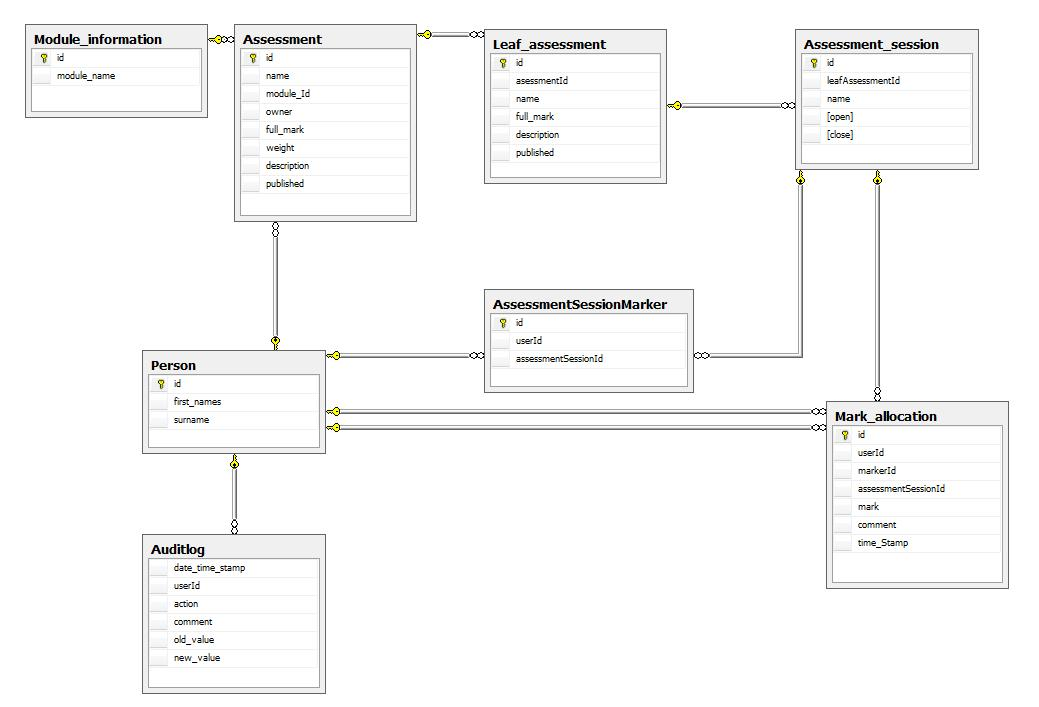
\includegraphics[scale=0.6]{./subdocs/Database/Database.jpg}}
\caption{Database Diagram}
\end{figure}

%Module information table
\begin{table}[ht]
\centering
\begin{tabular}[c]{|l|l|l|l|l|l|}
  \hline
  \multicolumn{6}{|c|}{Module\_Information} \\
  \hline 
  Field & Type & Null & Key & Default & Extra \\ [0.5ex] % Table Heading
  \hline
  id & int(11) & No & Pri & NULL & auto\_increment \\
  name & varchar(255) & No & & & \\
  \hline
\end{tabular}
\end{table} 

%Person table
\begin{table}[ht]
\begin{tabular}[c]{|l|l|l|l|l|l|}
  \hline
  \multicolumn{6}{|c|}{Person} \\
  \hline 
  Field & Type & Null & Key & Default & Extra \\ [0.5ex] % Table Heading
  \hline
  id & int(8) & No & Pri & NULL & auto\_increment \\
  first\_names & varchar(255) & Yes & & NULL & \\
  surname & varchar(255) & No & & & \\
  \hline
\end{tabular}
\end{table} 

%Auditlog table
\begin{table}[ht]
\begin{tabular}[c]{|l|l|l|l|l|l|}
  \hline
  \multicolumn{6}{|c|}{Auditlog} \\
  \hline 
  Field & Type & Null & Key & Default & Extra \\ [0.5ex] % Table Heading
  \hline
  date\_time\_stamp & datetime & No & & 0000\_00\_00 00:00:00 & \\
  id & int(8) & No & Foreign & & References Person \\
  action & varchar(20) & No & & & See reference 1 \\
  description & varchar(100) & Yes & & NULL & \\
  old\_value & varchar(100) & Yes & & NULL & \\
  new\_value & varchar(100) & No & & & \\
  \hline
\end{tabular}
\end{table} 

\newpage
{Reference 1: Action may have one of the following values: Assessment Created, Assessment Modified, Assessment Removed, Mark Submitted, Mark Modified, Mark Removed, Open Assessment, Close Assessment, Publish Marks, Assessment Report, Students Marks Report, Audit Report.}

%Assessment table
\begin{table}[ht]
\begin{tabular}[c]{|l|l|l|l|l|l|}
  \hline
  \multicolumn{6}{|c|}{Assessment} \\
  \hline 
  Field & Type & Null & Key & Default & Extra \\ [0.5ex] % Table Heading
  \hline
  id & int(8) & No & Pri & NULL & auto\_increment \\
  name & varchar(100) & No & & & \\
  moduleId & int(8) & No & Foreign & & References Module\_information \\
  owner & int(8) & No & Foreign & & References Person \\
  full\_mark & int(3) & No & & & \\
  weight & int(3) & Yes & & 100 & \\
  description & varchar(255) & Yes & NULL & & \\
  published & bit & No & & False & \\
  \hline
\end{tabular}
\end{table} 

%Leaf_assessment table
\begin{table}[ht]
\begin{tabular}[c]{|l|l|l|l|l|l|}
  \hline
  \multicolumn{6}{|c|}{Leaf\_assessment} \\
  \hline 
  Field & Type & Null & Key & Default & Extra \\ [0.5ex] % Table Heading
  \hline
  id & int(8) & No & Pri & NULL & auto\_increment \\
  assessmentId & int(8) & No & Foreign & & References Assessment \\
  name & varchar(100) & No & & & \\
  full\_mark & int(3) & No & & & \\
  description & varchar(255) & Yes & NULL & & \\
  published & bit & No & & False & \\
  \hline
\end{tabular}
\end{table} 

%Assessment_session table
\begin{table}[ht]
\begin{tabular}[c]{|l|l|l|l|l|l|}
  \hline
  \multicolumn{6}{|c|}{Assessment\_session} \\
  \hline 
  Field & Type & Null & Key & Default & Extra \\ [0.5ex] % Table Heading
  \hline
  id & int(8) & No & Pri & NULL & auto\_increment \\
  leafAssessmentId & int(8) & No & Foreign & & References Leaf\_assessment \\
  name & varchar(100) & No & & & \\
  open & datetime & No & & Date/time now & \\
  close & datetime & No & & Date/time now & \\
  \hline
\end{tabular}
\end{table} 

%Assessment_Session_Marker table
\begin{table}[ht]
\begin{tabular}[c]{|l|l|l|l|l|l|}
  \hline
  \multicolumn{6}{|c|}{Assessment\_Session\_Marker} \\
  \hline 
  Field & Type & Null & Key & Default & Extra \\ [0.5ex] % Table Heading
  \hline
  id & int(8) & No & Pri & NULL & auto\_increment \\
  userId & int(8) & No & Foreign & & References Person\\
  assessmentSessionId & int(8) & No & Foreign & & References Assessment\_session \\
  \hline
\end{tabular}
\end{table} 

%Mark_allocation table
\begin{table}[ht]
\begin{tabular}[c]{|l|l|l|l|l|l|}
  \hline
  \multicolumn{6}{|c|}{Mark\_allocation} \\
  \hline 
  Field & Type & Null & Key & Default & Extra \\ [0.5ex] % Table Heading
  \hline
  id & int(8) & No & Pri & NULL & auto\_increment \\
  userId & int(8) & No & Foreign & & References Person\\
  markerId & int(8) & No & Foreign & & References Person\\
  assessment\_session\_id & int(8) & No & Foreign & & References Assessment\_session \\
  mark & int(3) & No & & & \\
  comment & varchar(255) & Yes & & & \\
  time\_stamp & datetime & No & & & \\
  \hline
\end{tabular}
\end{table} 


